% Przykład eksportu TikZ (FB13) — eksport TikZ z mNotes
\documentclass[tikz,border=4pt]{standalone}
\usepackage[T1]{fontenc}
\begin{document}
% strona 1
% mNotes: rysunek w skali 1:1 (cm). Mniejszy: [scale=0.5, every node/.style={scale=0.5}]
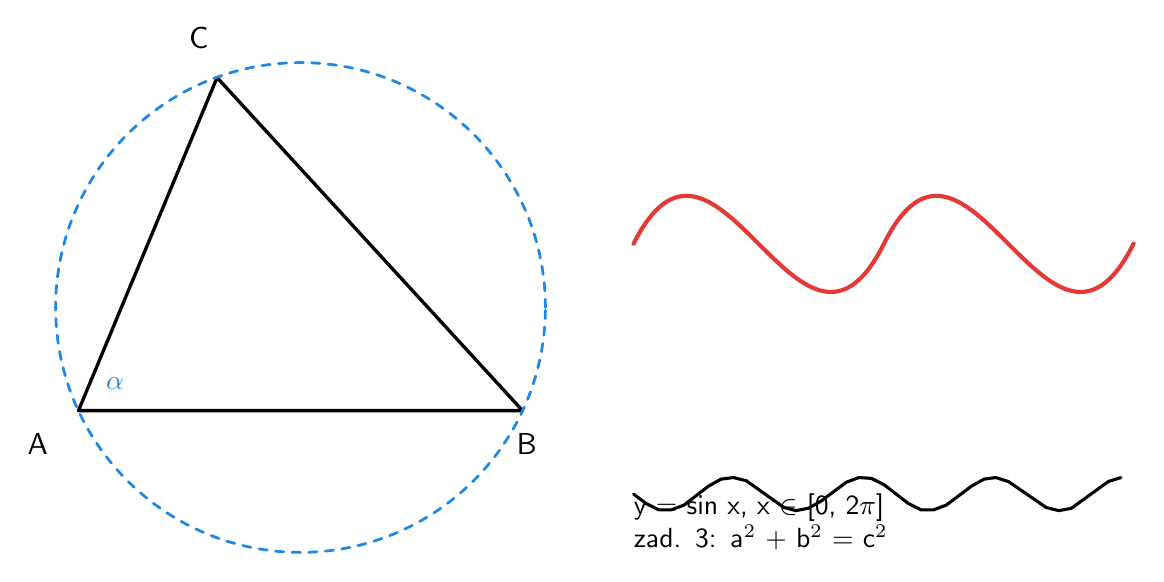
\begin{tikzpicture}[line cap=round, line join=round]
\definecolor{mn1}{HTML}{1E88E5}
\definecolor{mn2}{HTML}{E53935}
\draw[black, line width=1.2pt] (0.64,1.94) -- (6.28,1.94) -- (2.4,6.17) -- cycle;
\draw[mn1, line width=1pt, dashed] (3.46,3.25) circle [radius=3.11];
\draw[mn2, line width=1.5pt] (7.69,4.06) .. controls (8.75,6.17) and (9.81,1.94) .. (10.87,4.06)
  .. controls (11.92,6.17) and (12.98,1.94) .. (14.04,4.06);
\draw[black, line width=1.12pt] (7.69,0.88) -- (7.85,0.76) -- (8.01,0.68) -- (8.17,0.68) -- (8.33,0.74) -- (8.64,0.98)
  -- (8.8,1.07) -- (8.96,1.09) -- (9.12,1.05) -- (9.6,0.71) -- (9.75,0.67) -- (9.91,0.7)
  -- (10.07,0.79) -- (10.39,1.03) -- (10.55,1.09) -- (10.71,1.08) -- (10.87,1) -- (11.18,0.76)
  -- (11.34,0.68) -- (11.5,0.68) -- (11.66,0.74) -- (11.98,0.98) -- (12.14,1.07) -- (12.29,1.09)
  -- (12.45,1.04) -- (12.93,0.71) -- (13.09,0.67) -- (13.25,0.7) -- (13.72,1.04) -- (13.88,1.09);
\node[text=black, anchor=center, inner sep=0pt, align=left, text width=0.71cm, font=\fontsize{11}{13.2}\selectfont\sffamily] at (0.35,1.52) {A};
\node[text=black, anchor=center, inner sep=0pt, align=left, text width=0.71cm, font=\fontsize{11}{13.2}\selectfont\sffamily] at (6.56,1.52) {B};
\node[text=black, anchor=center, inner sep=0pt, align=left, text width=0.71cm, font=\fontsize{11}{13.2}\selectfont\sffamily] at (2.4,6.67) {C};
\node[text=mn1, anchor=center, inner sep=0pt, align=left, text width=1.06cm, font=\fontsize{10}{12}\selectfont\sffamily] at (1.52,2.29) {$\alpha$};
\node[text=black, anchor=center, inner sep=0pt, align=left, text width=6.35cm, font=\fontsize{10}{12}\selectfont\sffamily] at (10.87,0.53) {y = sin x, x $\in$ [0, 2$\pi$]\\ zad. 3: a$^{2}$ + b$^{2}$ = c$^{2}$};
\end{tikzpicture}
\end{document}
